\documentclass[twoside, openright, 11pt]{report}
\usepackage[spanish]{babel}
\usepackage[utf8]{inputenc}
\usepackage{graphicx}
\usepackage{listings}
\usepackage{color}

\begin{document}

\begin{titlepage}
\newlength{\centeroffset}
\setlength{\centeroffset}{-0.5\oddsidemargin}
\addtolength{\centeroffset}{0.5\evensidemargin}
\thispagestyle{empty}
\noindent\hspace*{\centeroffset}\begin{minipage}{\textwidth}
\centering

\includegraphics[width=0.9\textwidth]{imagenes/logo_ugr}\\[1.4cm]
\textsc{ \Large TRABAJO FIN DE GRADO\\[0.2cm]}
\textsc{ GRADO DE INGENIERÍA EN INFORMÁTICA}\\[1cm]
{\huge\bfseries NutriPlan\\}
\noindent\rule[-1ex]{\textwidth}{3pt}\\[3.5ex]
{\large\bfseries Aplicación para la Gestión de Recetas}
\end{minipage}

\vspace{0.5cm}
\noindent\hspace*{\centeroffset}\begin{minipage}{\textwidth}
\centering
\textbf{Autor}\\ Aissa Rouk El Masoudi\\[2.5ex]
\textbf{Directores}\\
Carlos Rodriguez Dominguez\\[2cm]

\includegraphics[width=0.3\textwidth]{imagenes/logo-ceuta.jpg}\\[0.1cm]
\textsc{Facultad de Educación, Tecnología y Economía de Ceuta}\\
\textsc{---}\\
Granada, 15 de Junio de 2025
\end{minipage}
\end{titlepage}
\let\cleardoublepage\clearpage

\chapter*{}
\begin{flushright}
\textit{Dedicado a\\
...}
\end{flushright}
\thispagestyle{empty}

\chapter*{Resumen}
\addcontentsline{toc}{chapter}{Resumen}
\markboth{RESUMEN}{RESUMEN}
\thispagestyle{empty}
En este trabajo se presenta el diseño y desarrollo de \textbf{NutriPlan}, una aplicación móvil multiplataforma para la gestión de recetas y la planificación semanal de menús. El proyecto surge de la necesidad de proporcionar a los usuarios una herramienta que les permita organizar de forma eficiente sus comidas, llevar un control nutricional y mejorar sus hábitos alimentarios mediante la digitalización de recetas. A lo largo del documento se describe el análisis del problema, la justificación de la tecnología empleada y las principales decisiones de diseño y desarrollo. Se exponen los requisitos funcionales y no funcionales, así como la arquitectura general de la solución basada en React Native, la estructura de datos utilizada y la interfaz de usuario. Finalmente se analizan los resultados obtenidos y se plantean posibles líneas de mejora y trabajos futuros.

\chapter*{Abstract}
\addcontentsline{toc}{chapter}{Abstract}
\markboth{ABSTRACT}{ABSTRACT}
\thispagestyle{empty}
This document presents the design and development of \textbf{NutriPlan}, a cross‑platform mobile application for recipe management and weekly meal planning. The project addresses the need for a tool that enables users to organize their meals efficiently, monitor their nutritional intake, and improve their eating habits through the digitalization of recipes. The report describes the problem analysis, the rationale behind the chosen technology and the main design and implementation decisions. It outlines the functional and non‑functional requirements, the system architecture based on React Native, the data structures employed and the user interface. The results are discussed and possible improvements and future work are proposed.

\tableofcontents

\cleardoublepage
\addcontentsline{toc}{chapter}{Lista de figuras}
\listoffigures

\cleardoublepage
\addcontentsline{toc}{chapter}{Lista de tablas}
\listoftables

\chapter{Introducción}\label{cap.introduccion}

\section{Motivación}
La planificación de las comidas diarias es una tarea compleja que requiere organizar recetas, estimar cantidades y garantizar una dieta equilibrada. En la actualidad existen numerosas aplicaciones que facilitan la obtención de recetas, pero pocas ofrecen al usuario un entorno integrado en el que pueda gestionar su propio recetario, planificar menús semanales y realizar un seguimiento nutricional personalizado. \textbf{NutriPlan} nace con el propósito de satisfacer estas necesidades proporcionando una herramienta intuitiva y accesible, aprovechando la ubiquidad de los dispositivos móviles y el potencial de las tecnologías multiplataforma.

\section{Objetivos}
Los objetivos de este trabajo se dividen en generales y específicos:
\begin{itemize}
  \item \textbf{Objetivo general}: desarrollar una aplicación multiplataforma que permita al usuario gestionar recetas y planificar sus comidas de forma sencilla, visualizando la información nutricional asociada y generando listas de la compra.
  \item \textbf{Objetivos específicos}: 
  \begin{itemize}
    \item Diseñar una arquitectura de software modular basada en React Native que facilite la extensibilidad y el mantenimiento del código.
    \item Implementar funcionalidades de creación, edición y eliminación de recetas, así como la asignación de recetas a cada día de la semana.
    \item Calcular y mostrar automáticamente los valores nutricionales de las recetas y del menú semanal.
    \item Generar una lista de compra en función del menú planificado.
    \item Proporcionar una interfaz gráfica atractiva y accesible, apoyada en mockups y pruebas con usuarios.
    \item Evaluar el rendimiento y la usabilidad de la aplicación mediante pruebas unitarias, de integración y con usuarios.
  \end{itemize}
\end{itemize}

\section{Estructura de la memoria}
El documento se organiza de la siguiente forma:
\begin{itemize}
  \item En el \textbf{Capítulo~\ref{cap.introduccion}} se presentan la motivación, objetivos, estructura y planificación del proyecto.
  \item El \textbf{Capítulo~\ref{cap.estado del arte}} analiza el estado del arte, revisando tecnologías y proyectos relacionados.
  \item En el \textbf{Capítulo~\ref{cap.diseno y descripcion del sistema}} se describen los requisitos, la arquitectura de la aplicación y las decisiones de diseño, incluyendo mockups de la interfaz.
  \item El \textbf{Capítulo~\ref{cap.prototipos y desarrollo}} detalla los prototipos desarrollados y la evolución de la aplicación.
  \item El \textbf{Capítulo~\ref{cap.conclusiones y mejoras futuras}} recoge las conclusiones, la valoración personal y las mejoras futuras.
  \item Finalmente se incluye un \textbf{capítulo en inglés} con las conclusiones y trabajos futuros y el listado de referencias bibliográficas.
\end{itemize}

\section{Recursos utilizados}
Para el desarrollo de \textbf{NutriPlan} se han empleado los siguientes recursos:
\begin{itemize}
  \item \textbf{Hardware}: ordenador portátil con procesador Intel i5 y 16~GB de RAM, dispositivo Android para pruebas y emulador iOS.
  \item \textbf{Software}: sistema operativo Ubuntu~22.04, Node.js~18, IDE Visual Studio Code, emuladores Android/iOS y sistemas de control de versiones Git. Para el desarrollo se utilizó \textbf{Expo} como entorno de ejecución de React Native.
  \item \textbf{Librerías y frameworks}: \verb|@react-navigation| para la gestión de la navegación, \verb|react-native-paper| para componentes de interfaz, \verb|redux| para la gestión del estado global, y \verb|async-storage| para el almacenamiento local. La aplicación fue tipada con TypeScript para mejorar la mantenibilidad del código.
  \item \textbf{Herramientas de documentación y edición}: \LaTeX{} para la redacción de la memoria, GitHub para la gestión de versiones y Canva para el diseño de mockups.
\end{itemize}

\section{Planificación temporal}
La planificación temporal del proyecto se llevó a cabo mediante un diagrama de Gantt en el que se establecieron las etapas principales: análisis y especificación de requisitos (2~semanas), diseño de la arquitectura y mockups (3~semanas), desarrollo incremental mediante prototipos (8~semanas), pruebas y optimización (3~semanas) y redacción de la memoria (3~semanas). Cada fase se revisó periódicamente para adaptarse a los resultados obtenidos y se documentó en el repositorio del proyecto.

\chapter{Estado del arte}\label{cap.estado del arte}
\section{Fundamentos}
La planificación de menús está estrechamente relacionada con la nutrición y la seguridad alimentaria. Distintas guías dietéticas —como la pirámide alimentaria o el plato Harvard— recomiendan distribuir los macronutrientes (hidratos de carbono, proteínas y grasas) de forma equilibrada y priorizar el consumo de frutas, verduras y cereales integrales. La digitalización de recetas permite obtener información nutricional precisa y adaptarla a las necesidades de cada usuario, favoreciendo la adopción de hábitos saludables.

\section{Análisis de librerías y frameworks para el desarrollo de aplicaciones móviles}
Para el desarrollo de aplicaciones móviles existen diversas alternativas. Las más extendidas son las aplicaciones nativas, que se desarrollan en \textbf{Java/Kotlin} para Android y \textbf{Swift/Objective‑C} para iOS, y las aplicaciones multiplataforma, basadas en frameworks como \textbf{Flutter} y \textbf{React Native}. Flutter ofrece un rendimiento próximo al nativo y un lenguaje declarativo (Dart) con gran consistencia visual, pero su comunidad en español es todavía limitada. React Native, por su parte, utiliza JavaScript o TypeScript y permite reutilizar componentes web, cuenta con una comunidad muy amplia y numerosas librerías de apoyo. Tras comparar ambas alternativas, se optó por React Native debido a su madurez, su ecosistema y su curva de aprendizaje moderada. Además, la utilización de \textbf{Expo} simplifica la configuración del entorno y la distribución en dispositivos reales.

\section{Análisis de librerías y frameworks para back‑end}
NutriPlan está diseñada como una aplicación sin servidor, centrada en el almacenamiento local. Para la persistencia de datos se utiliza \verb|AsyncStorage|, que permite guardar información en el dispositivo del usuario, y se contempla la posibilidad de integrar bases de datos ligeras como \verb|SQLite| mediante \verb|expo-sqlite|. Sin embargo, se realizó un análisis de frameworks back‑end para evaluar la escalabilidad futura. \textbf{Node.js} con \textbf{Express} resulta apropiado para aplicaciones REST por su eficiencia y flexibilidad; \textbf{Django} en Python destaca por sus funcionalidades integradas y su robustez; y \textbf{Firebase} ofrece soluciones de autenticación y base de datos en tiempo real sin mantenimiento de servidores. La elección de un back‑end dependerá de los requisitos de sincronización y colaboración multiusuario en versiones futuras.

\section{Proyectos actuales}
Existen numerosas aplicaciones comerciales dedicadas a la planificación de comidas y recetas, como \textit{Yummly}, \textit{Paprika} o \textit{Cookpad}. Estas aplicaciones permiten buscar recetas, gestionar listas de compra y en algunos casos planificar menús semanales. Sin embargo, muchas de ellas requieren suscripciones, carecen de soporte en español o no ofrecen una integración completa de la información nutricional. NutriPlan se inspira en estas soluciones, pero se centra en la personalización y en la posibilidad de que el usuario cree y modifique su propio recetario.

\section{Conclusiones}
El estudio del estado del arte muestra que React Native es una opción adecuada para desarrollar aplicaciones multiplataforma debido a su madurez y su comunidad. Asimismo, aunque actualmente el proyecto no requiere un back‑end, la evaluación de tecnologías como Node.js, Django y Firebase permitirá escalar la aplicación en futuras versiones. NutriPlan pretende diferenciarse de las aplicaciones existentes ofreciendo una plataforma gratuita, en español y centrada en el usuario.

\chapter{Diseño y descripción del sistema}\label{cap.diseno y descripcion del sistema}
\section{Requisitos funcionales y no funcionales}
\subsection{Requisitos funcionales}
\begin{itemize}
  \item RF1: El sistema debe permitir al usuario registrar, editar y eliminar recetas con sus ingredientes, cantidades y procedimiento.
  \item RF2: El usuario puede asignar recetas a cada día de la semana, generando un plan de comidas.
  \item RF3: La aplicación debe calcular automáticamente los valores nutricionales de cada receta y del menú semanal, mostrando calorías, proteínas, hidratos y grasas.
  \item RF4: Debe generar una lista de la compra agregada según las recetas programadas para la semana.
  \item RF5: Se debe poder buscar y filtrar recetas por nombre, ingredientes o etiquetas.
  \item RF6: La aplicación almacenará la información de forma local, permitiendo su uso sin conexión.
\end{itemize}
\subsection{Requisitos no funcionales}
\begin{itemize}
  \item RNF1: La interfaz debe ser intuitiva y accesible, cumpliendo las directrices de diseño de Material Design.
  \item RNF2: El sistema debe estar disponible en dispositivos Android e iOS.
  \item RNF3: El tiempo de respuesta en las operaciones principales debe ser inferior a 200~ms.
  \item RNF4: Se debe garantizar la persistencia de datos aunque el usuario cierre la aplicación.
  \item RNF5: El código debe ser modular y documentado para facilitar su mantenimiento.
\end{itemize}

\section{Arquitectura de la aplicación}
La arquitectura de NutriPlan sigue un patrón \textbf{modelo‑vista‑controlador} adaptado a React Native. El código se organiza en directorios claros: \verb|/components| contiene componentes presentacionales reutilizables como botones, tarjetas de receta o campos de texto; \verb|/screens| alberga las pantallas principales de la aplicación (lista de recetas, detalles, plan semanal, perfil); \verb|/services| agrupa la lógica de acceso a datos y cálculos nutricionales; \verb|/navigation| define los navegadores de pila (\textit{stack}) y pestañas (\textit{tabs}) mediante \verb|@react-navigation|; y \verb|/store| implementa la gestión de estado con Redux. La figura~\ref{fig:arquitectura} muestra un diagrama de componentes simplificado.

\begin{figure}[h]
  \centering
  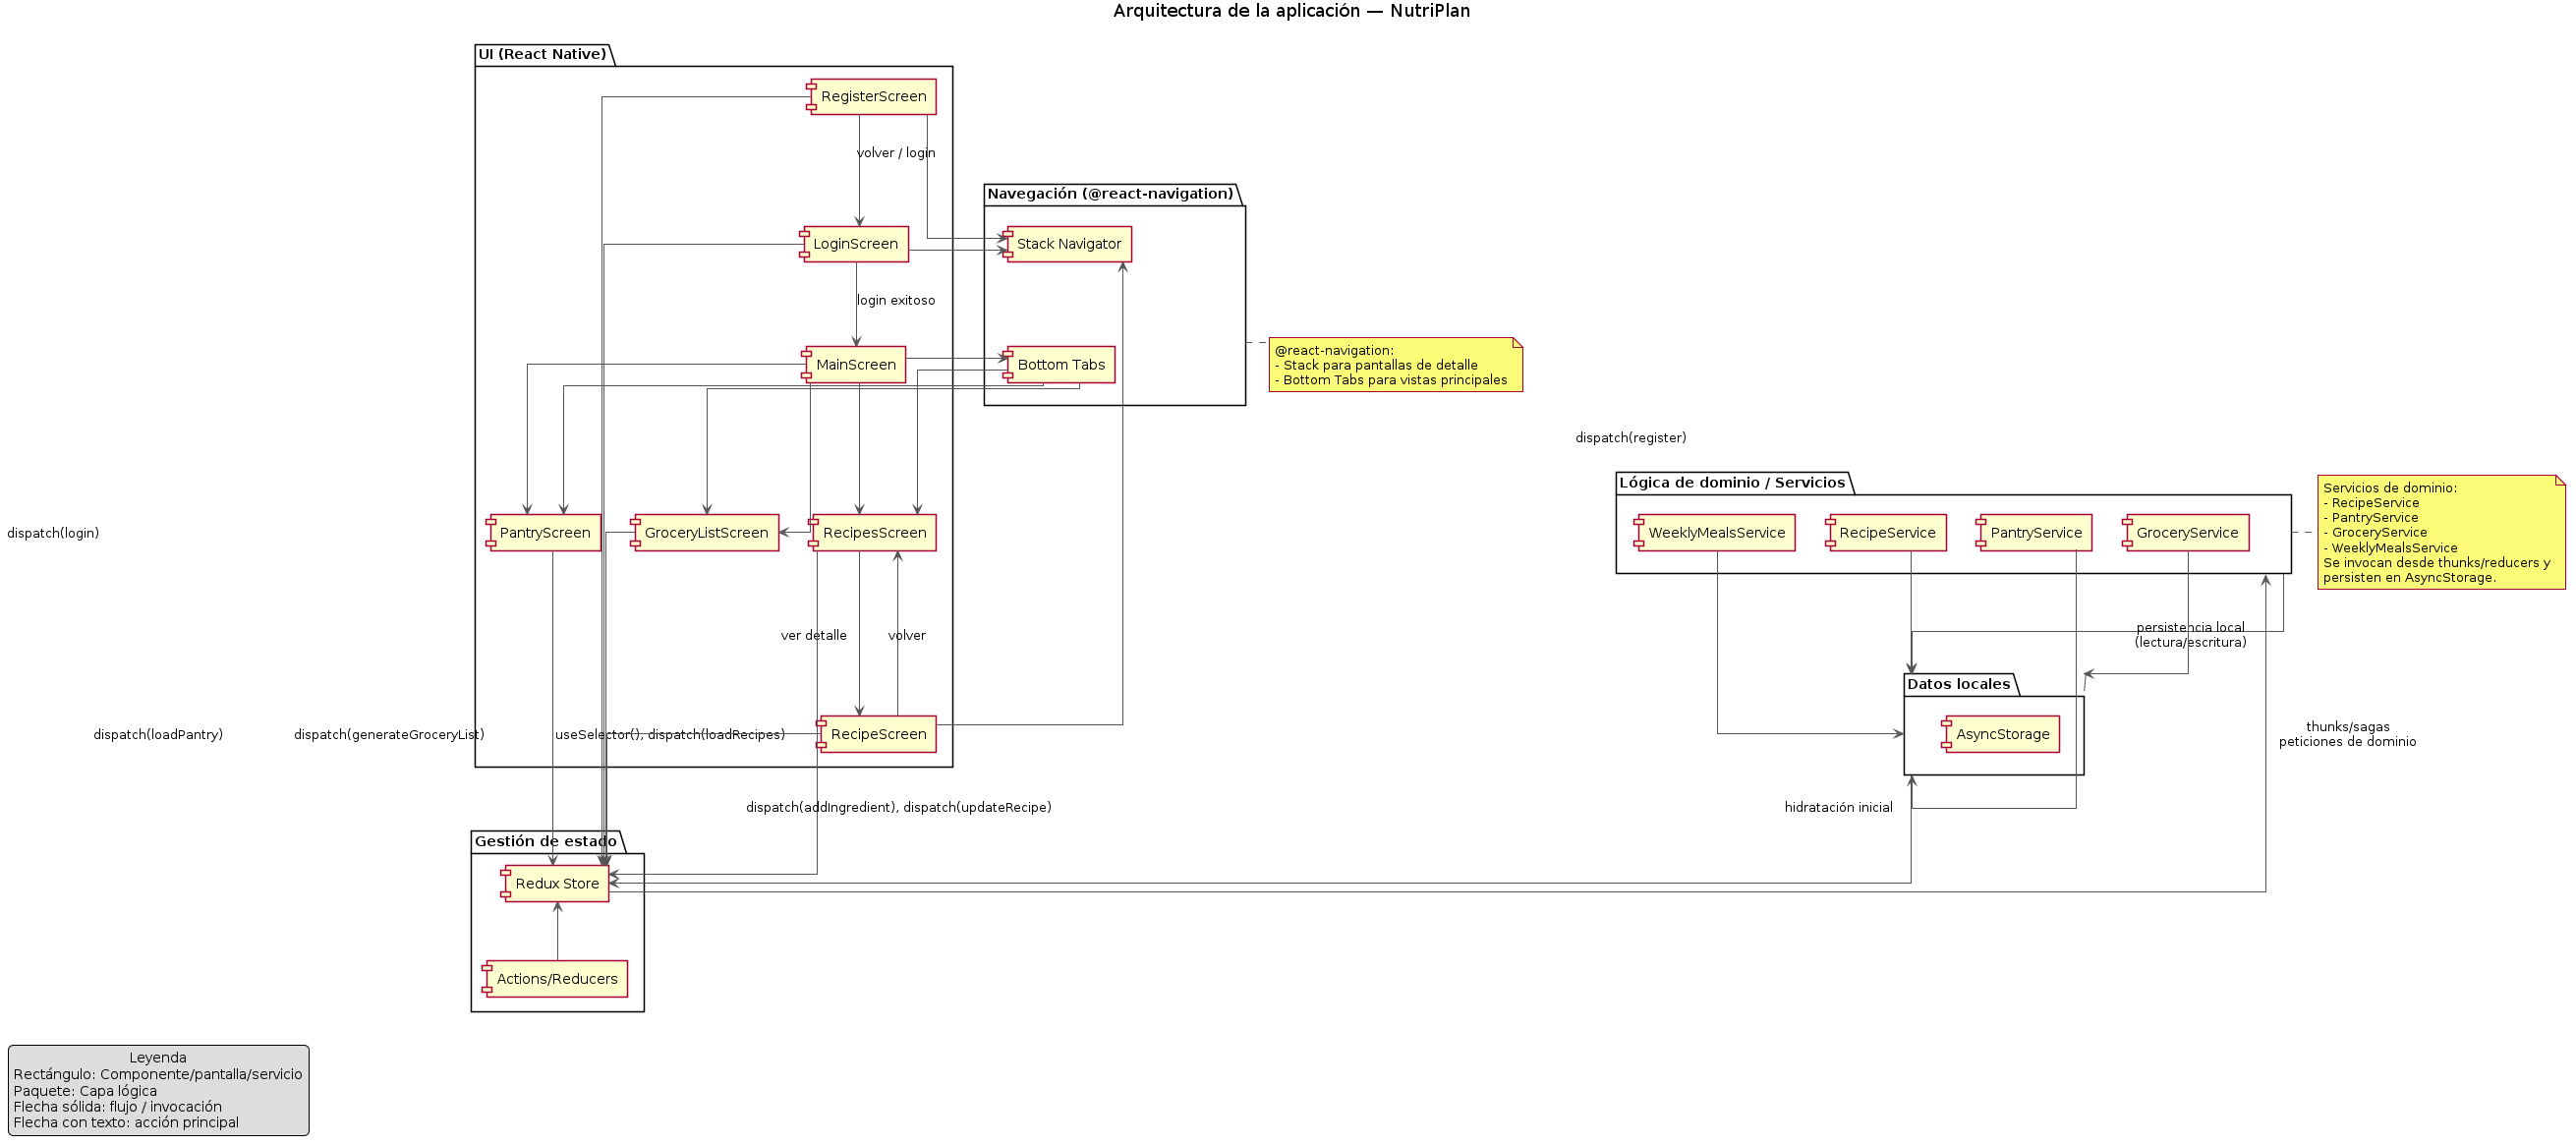
\includegraphics[width=0.8\textwidth]{imagenes/arquitectura.png}
  \caption{Arquitectura de la aplicación NutriPlan.}
  \label{fig:arquitectura}
\end{figure}

El uso de \textbf{Redux} facilita la actualización reactiva de la interfaz y la compartición de datos entre pantallas. Las acciones (por ejemplo, \texttt{addRecipe} o \texttt{assignRecipeToDay}) disparan cambios en el \emph{store} y los componentes se actualizan automáticamente mediante el hook \verb|useSelector|. La navegación se gestiona mediante \verb|createBottomTabNavigator| para las pestañas principales (Recetas, Plan semanal, Lista de la compra) y \verb|createStackNavigator| para navegar a las pantallas de detalles.

\section{Modelo de datos}
Los datos se estructuran en tres entidades principales:
\begin{description}
  \item[Receta:] contiene identificador, nombre, descripción, lista de ingredientes (nombre, cantidad, unidad), pasos de preparación, información nutricional por porción y etiquetas.
  \item[Plan de comidas:] almacena la asignación de recetas a los días de la semana y permite calcular la suma de nutrientes.
  \item[Lista de compra:] genera una colección de ingredientes agregados con su cantidad total según el plan de comidas.
\end{description}
Estas entidades se representan mediante interfaces de TypeScript que facilitan el tipado y la consistencia de los datos en toda la aplicación.

\section{Mockups}
El diseño de la interfaz se definió a partir de un conjunto de \emph{mockups} realizados con la herramienta Figma. Se siguieron los principios de Material Design: uso de tarjetas para agrupar información, colores neutros y acentos en verde para representar lo saludable, y jerarquía tipográfica clara. La figura~\ref{fig:mockup_lista} muestra el mockup de la lista de recetas. Las pantallas comparten un menú de navegación inferior que permite acceder rápidamente a las funciones principales. Durante el desarrollo se realizaron pruebas con usuarios para evaluar la usabilidad y se introdujeron mejoras como la reorganización de botones y el uso de iconos intuitivos.

\begin{figure}[h]
  \centering
  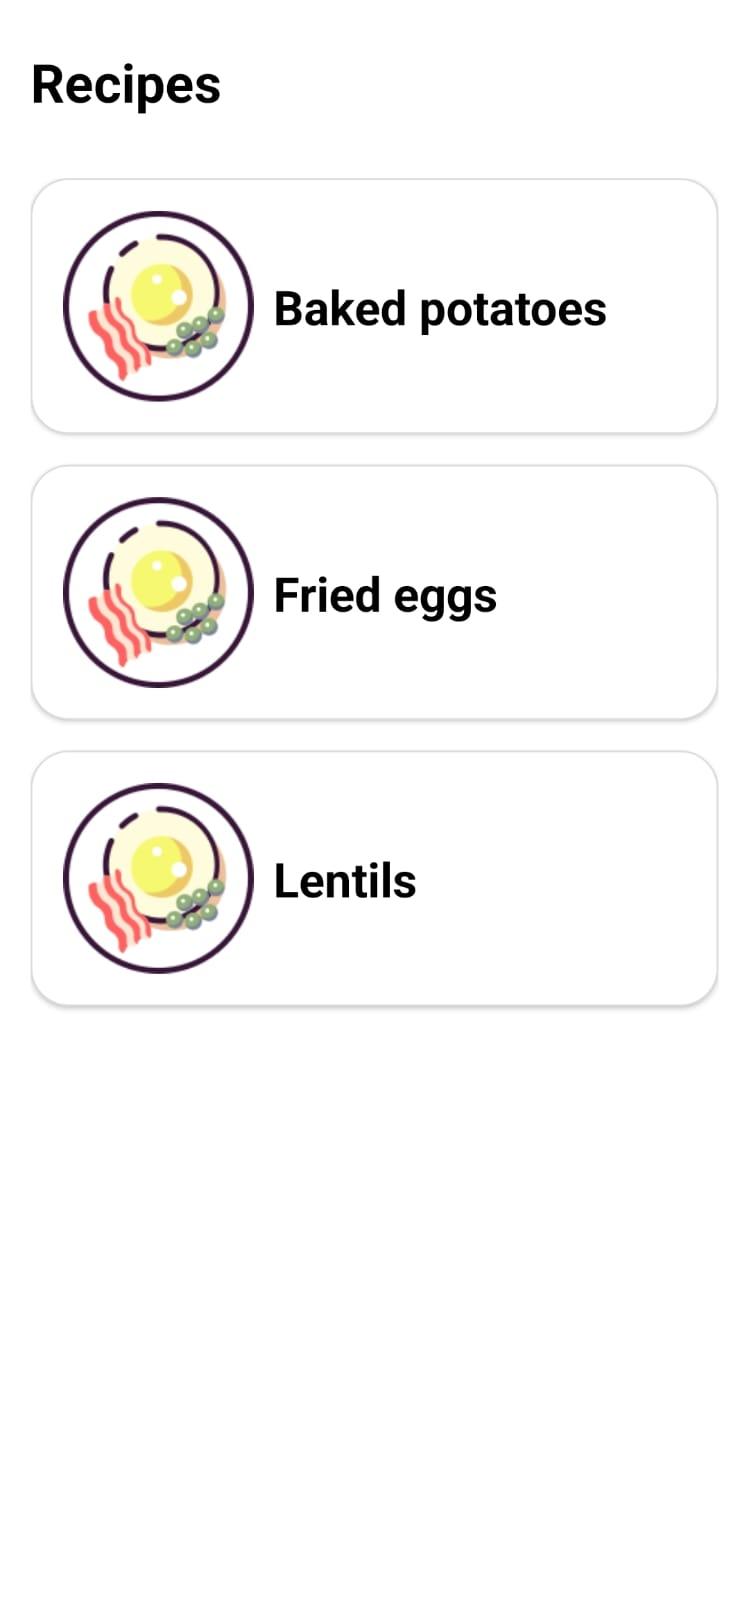
\includegraphics[width=0.5\textwidth]{imagenes/RecipesScreen.jpeg}
  \caption{Mockup de la pantalla de lista de recetas.}
  \label{fig:mockup_lista}
\end{figure}

\section{Conclusiones}
El diseño del sistema responde a la necesidad de modularidad y escalabilidad, organizando el código en capas bien definidas. La utilización de Redux y React Navigation simplifica el flujo de datos y la navegación, mientras que el almacenamiento local garantiza la disponibilidad sin conexión. La implementación de interfaces intuitivas basadas en principios de diseño mejora la experiencia de usuario.

\chapter{Prototipos y desarrollo}\label{cap.prototipos y desarrollo}

El desarrollo de NutriPlan se llevó a cabo de forma incremental mediante tres prototipos principales.

\section{Prototipo 1}
En el primer prototipo se creó la estructura básica de la aplicación, configurando el entorno con Expo y React Native. Se implementó la navegación con \verb|createBottomTabNavigator| y se desarrollaron pantallas simples para la lista de recetas y el plan semanal. Se añadieron componentes reutilizables para botones y tarjetas.

\section{Prototipo 2}
El segundo prototipo añadió la funcionalidad de creación y edición de recetas. Se integró Redux para la gestión del estado y se implementó la persistencia local con \verb|AsyncStorage|. Se creó un formulario con validación para introducir ingredientes y pasos, y se mostraron cálculos nutricionales utilizando una librería de nutrición. Asimismo se diseñó la pantalla de detalles de receta con secciones desplegables.

\section{Prototipo 3}
El tercer prototipo incorporó la generación de la lista de la compra y la planificación semanal. Se añadieron funciones para asignar recetas a cada día, sumar los ingredientes necesarios y presentar una lista organizada por categorías. Se mejoró la interfaz con animaciones sutiles y se realizaron pruebas de usabilidad con un grupo de usuarios, cuyos comentarios llevaron a ajustes en la navegación y en la presentación de la información.

\section{Conclusiones}
La evolución por prototipos permitió ajustar el alcance y mejorar la aplicación de forma continua. Cada iteración se validó mediante pruebas unitarias y con usuarios. Al finalizar el desarrollo, la aplicación ofrece un conjunto coherente de funcionalidades que satisfacen los objetivos propuestos y constituyen una base sólida para futuras ampliaciones.

\chapter{Conclusiones y mejoras futuras}\label{cap.conclusiones y mejoras futuras}

\section{Conclusiones técnicas}
El desarrollo de NutriPlan ha puesto de manifiesto la idoneidad de React Native para construir aplicaciones multiplataforma con un único código base. El uso de Redux y TypeScript ha facilitado la escalabilidad y el mantenimiento, mientras que la persistencia local proporciona independencia de un servidor externo. Las pruebas realizadas demuestran que la aplicación responde adecuadamente y ofrece una experiencia fluida al usuario. Sin embargo, será necesario optimizar la gestión de estados complejos si se incorporan nuevas funcionalidades.

\section{Conclusiones personales}
A nivel personal, la realización de este proyecto ha supuesto una oportunidad para profundizar en el desarrollo móvil y en la organización de proyectos de software. La elección de tecnologías y la planificación detallada han sido clave para alcanzar los objetivos. Asimismo se han desarrollado habilidades en diseño de interfaces, documentación y comunicación de resultados.

\section{Futuras mejoras}
Entre las mejoras futuras se contemplan:
\begin{itemize}
  \item Implementar un sistema de autenticación para sincronizar datos entre dispositivos y permitir compartir recetas entre usuarios.
  \item Integrar una base de datos externa (por ejemplo Firebase o MongoDB) para almacenar recetas en la nube.
  \item Añadir funcionalidades de búsqueda avanzada y filtrado por valores nutricionales.
  \item Incorporar un módulo de recomendaciones basado en los hábitos del usuario y preferencias alimentarias.
  \item Desarrollar pruebas automatizadas (unitarias, de integración y de interfaz) para incrementar la fiabilidad del sistema.
\end{itemize}

\chapter{Conclusions and future works}\label{cap.conclusions and future works}
\section{Technical conclusions}
The development of NutriPlan demonstrates that React Native is well suited for cross‑platform mobile applications. Redux and TypeScript contributed to maintainable and scalable code, while local persistence provided an offline capability. Further improvements may address the management of complex states and the integration of online services.

\section{Personal conclusions}
From a personal perspective, this project has provided valuable experience in mobile development, project planning and user interface design. It has also highlighted the importance of incremental development and continuous testing.

\section{Future works}
Future work may include authentication and cloud synchronization, enhanced nutritional analysis features and the implementation of automated testing. Extending the app to support multiuser collaboration and dietary recommendations would also add value.

\cleardoublepage
\addcontentsline{toc}{chapter}{Bibliografía}
\bibliographystyle{acm}
\bibliography{citas}

\end{document}
